\section{Theorie}

Das Ziel des Versuches ist es, die longitudinale bzw. Spin-Gitter-Relaxationszeit, sowie die
transversale bzw. Spin-Spin-Relaxationszeit von bidestilierten Wasser
mit Hilfe der Kernspinresonanz (NMR) zu bestimmen.

\subsection{Magentisierung im thermischen Gleichgewicht}

Durch das Anlegen eines Magnetfeldes werden entarteten Kenspinzustände
der Spinquantenzahl \textbf{I} in $2\text{\textbf{I}} + 1$ äquidistante
Unternivaus aufgespalten.
Die aufgespaltenen Niveaus werden durch die Orientierungsquantenzahl $m$
($-\text{\textbf{I}} \leq m \leq \text{\textbf{I}}$) unterschieden.
Benachbarte Energieniveaus haben einen Abstand von $\Delta E = \gamma B_0\hbar$,
wobei $\gamma$ das gyromagnetische Moment und somit das Verhältnis von
Drehimpuls oder Spin zu dem magnetischen Moment $\vec{\mu}$ darstellt.
Thermisch sind die Energieniveaus gemäß der Boltzmann-Verteilung
besetzt. Das Besetzungsverhältnis zweier benachbarter Energiezustände bei Temperatur $T$
hat folglich die Gestalt
\begin{equation}
  \label{eqn:boltzmann}
  \frac{N(m)}{N(m-1)} = \exp{\left(-\beta(T)\gamma B_0\hbar\right)},\qquad\text{mit }\beta(T) = \frac{1}{k\ua{B}T}.
\end{equation}

Der Erwartungswert der Kernspinpolarisation relativ zu dem angelegten Magnetfeld
$\braket{\text{\textbf{I}}\ua{z}}$ wird gemäß

\begin{equation}
  \label{eqn:erwartung_I}
  \braket{\text{\textbf{I}}\ua{z}} = \frac{\sum_{m = -\text{\textbf{I}}}^\text{\textbf{I}}
  \hbar m \exp{\left(-m\beta(T)\gamma B_0 \hbar\right)}}{\sum_{m = -\text{\textbf{I}}}^\text{\textbf{I}}
  \exp{\left(-m\beta(T)\gamma B_0 \hbar\right)}}
\end{equation}

beschrieben. Die folgenden Rechnungen beschränken sich auf die Vereinfachung
$\text{\textbf{I}} = \frac{1}{2}$, sowie große Magnetfelder $B_0 ~ \SI{1}{\tesla}$.
Dadurch gilt $m\beta(T)\gamma B_0\hbar \ll 1$, weshalb eine Linearisierung der
Exponentialfunktion in Formel~\ref{eqn:erwartung_I} gerechtfertigt ist.
Eine Darstellung der Energieniveaus ist in Abbildung~\ref{fig:proton} zu finden.

\begin{figure}
  \centering
  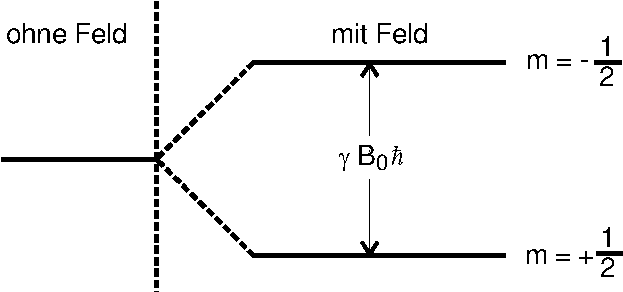
\includegraphics[width = 0.7\textwidth]{Pics/aufspaltungE}
  \caption{Energiezustände eines Protons ($\text{\textbf{I}} = \frac{1}{2}$) im Magnetfeld $B_0$\cite{anleitung}.}
  \label{fig:proton}
\end{figure}

Die Linearisierung von Formel~\ref{eqn:erwartung_I} ergibt
\begin{equation}
  \label{eqn:I_linear}
  \braket{\text{\textbf{I}}_{z} = \frac{1}{2}} = -\frac{\hbar^2}{4}\beta(T)\gamma B_0.
\end{equation}

Die Spinpolarisation führt eine Ausrichtung der mit dem Spin gekoppelten magnetischen
Momente $\vec{\mu}_\text{\textbf{I}}$ mit sich, woher eine makroskopische Magnetisierung
$\vec{M_0}$ rührt.
Liegen $N$ Momente $\vec{\mu}$ in der betrachteten Probe, kann der Betrag der
Magnetisierung $M_0$ geschrieben werden als
\begin{equation}
  \label{eqn:mag}
  M_0 = \frac{1}{4}\mu_0\gamma^2\frac{\hbar^2}N B_0\beta(T).
\end{equation}

\subsection{Lamor-Präzession}
Die magnetischen Momente führen um die Achse des angelegten Magnetfeldes
eine Präzessionsbewegung aus, welche als Lamor-Präzession bezeichnet wird.
Aus der Verbindung zwischen dem Gesamtdrehimpuls und der Magnetisierung
ergibt sich der folgende Zusammenhang.

\begin{equation}
  \label{eqn:mag_diff}
  \frac{\su{d}\vec{M}}{\su{d}t} = \gamma\vec{M}\times B_0\vec{e}_z
\end{equation}

Dabei ist $\vec{e}_z$ der Einheitsrichtungsvektor des Magnetfeldes.
Die Zerlegung von $\vec{M}$ in Einheitsvektoren eines karthesischen Systems
$\vec{e}_x, \vec{e}_y, \vec{e}_z$ führt auf drei Differentialgleichungen.

\begin{align}
  \label{eqn:M_x}
  \frac{\su{d}\vec{M}}{\su{d}t}\cdot \vec{e}_x &= \gamma B_0 \vec{M}\cdot \vec{e}_y, \\
  \label{eqn:M_y}
  \frac{\su{d}\vec{M}}{\su{d}t}\cdot \vec{e}_y &= -\gamma B_0 \vec{M}\cdot \vec{e}_x, \\
  \label{eqn:M_z}
  \frac{\su{d}\vec{M}}{\su{d}t}\cdot \vec{e}_z &= 0
\end{align}

Die Gleichungen~\ref{eqn:M_x}~bis~\ref{eqn:M_z} werden gelöst durch
\begin{align*}
  \vec{M}\cdot \vec{e}_x &= A\cos{(\gamma B_0 t)},\\
  \vec{M}\cdot \vec{e}_y &= -A\sin{(\gamma B_0 t)},\\
  \vec{M}\cdot \vec{e}_z &= \text{const},
\end{align*}
woran erkenntlich wird, dass die Magnetisierung $\vec{M}$ eine Präzession
um $\vec{e}_z$ mit der Lamor-Frequenz $\omega\ua{L} = \gamma B_0$ ausführt.

\subsection{Relaxationserscheinungen}

Relaxation tritt auf, wenn ein System aufgrund einer zeitlich begrenzten
Störung aus dem Gleichgewichtszustand gebracht wird.
In diesem Versuch wird solch eine Störung mit Hilfe hochfrequenter
Strahlungsquanten realisiert.
Eine Relaxation lässt sich durch eine Abwandlung der Gleichungen~\ref{eqn:M_x}~bis~\ref{eqn:M_z}
mathematisch wie folgt beschreiben

\begin{align}
  \label{eqn:M_x_relax}
  \frac{\su{d}\vec{M}}{\su{d}t}\cdot \vec{e}_x &= \gamma B_0 \vec{M}\cdot \vec{e}_y-\frac{1}{T_2}\vec{M}\cdot \vec{e}_x, \\
  \label{eqn:M_y_relax}
  \frac{\su{d}\vec{M}}{\su{d}t}\cdot \vec{e}_y &= -\gamma B_0 \vec{M}\cdot \vec{e}_x-\frac{1}{T_2}\vec{M}\cdot \vec{e}_y, \\
  \label{eqn:M_z_relax}
  \frac{\su{d}\vec{M}}{\su{d}t}\cdot \vec{e}_z &= \frac{1}{T_1}\left(M_0 - \vec{M}\cdot \vec{e}_z\right).
\end{align}

Die in den Gleichungen auftretenden Zeitkonstanten $T_1$ und $T_2$ sind
verschiedene Relaxationszeiten.
\begin{description}
  \item[Spin-Gitter-Relaxationszeit/longitudinal:]Relaxationszeit parallel zur Magnetfeldrichtung $T_1$.
  Charakteristische Übergangszeit von Energie des Kernspins in Gitterschwingungen und umgekehrt.
  \item[Spin-Spin-Relaxationszeit/transversal:]Relaxationszeit senkrecht zur Magnetfeldrichtung $T_2$.
  Hauptsächlich durch Spinwechselwirkungen mit den nächsten Nachbarn hervorgerufen. Es können
  aber auch Spin-Gitter-Relaxationsprozesse zu $T_2$ beitragen.
\end{description}

\subsection{Einstrahlung von HF-Strahlungsquanten}

Die Strahlungsquanten werde zur Auslenkung der
Probenmagnetisierung aus der Gleichgewichtslage verwendet.
Das hochfrequente Strahlungsfeld ist so ausgerichtet, dass es senkrecht zu dem Magnetfeld
$\vec{B_0}$ und somit senkrecht zu $\vec{e}_z$ steht.
\begin{equation}
  \label{eqn:hochfrequent}
  \vec{B}\ua{HF} = 2\vec{B}_1 \cos{(\omega t)}
\end{equation}

Eine Transformation in ein mit $\omega$ um die $\vec{e}_z$-Achse
bewegtes Koordinatensystem führt dazu, dass die Zeitabhängigkeit
in $\vec{B}_1$ eliminiert wird. Die Zeitabhängigkeit wird
somit in den Einheitsvektoren eingebunden, sodass ein Übergang
von $\left\{\vec{e}_x, \vec{e}_y, \vec{e}_z\right\}$ in
$\left\{\vec{e}'_x, \vec{e}'_y, \vec{e}'_z\right\}$ statt findet.
Die zeitliche Änderung der Magnetisierung transformiert sich zu
\begin{equation}
  \label{eqn:mag_trafo}
  \frac{\su{d}\vec{M}}{\su{d}t} = \gamma\left\{\vec{M}\times\left(\vec{B} + \frac{\vec{\omega}}{\gamma}\right)\right\}.
\end{equation}
Das Einführen eines effektiven Magnetfeldes $\vec{B}\ua{eff} = \vec{B}_0 + \vec{B}_1 + \frac{\vec{\omega}}{\gamma}$
vereinfacht Gleichung~\ref{eqn:mag_trafo} wie folgt:
\begin{equation}
  \label{eqn:B_eff}
  \frac{\su{d}\vec{M}}{\su{d}t} =\gamma\left(\vec{M}\times\vec{B}\ua{eff}\right).
\end{equation}
Der Resonanzfall der Störung tritt auf, wenn die Einstrahlfrequenz $\omega$
gleich der Lamorfrequenz $\omega\ua{L}$ ist.
Da $\vec{\omega}$ antiparallel zu $\vec{e}_z$ steht, ist
das effektive Magnetfeld $\vec{B}\ua{eff} = \vec{B}_1$.
Das bedeutet, dass die Magnetisierung um die $\vec{B}$- Achse präzidiert.

Soll die Magnetisierung $\vec{M}$ um 90° aus der $\vec{e}_z$-Achse
herausgedreht werden muss die Einstrahlungszeit
\begin{equation}
  \label{eqn:90grad}
  \Delta t_{90} = \frac{\pi}{2\gamma B_1}
\end{equation}
betragen. Eine Drehung um 180° bedarf einer Einstrahlzeit von
$2\cdot\Delta t_{90}$.
Im Folgenden wird eine Drehung um 90° als 90°-Puls und eine
Drehung um 180° als 180°-Puls bezeichnet.

\subsection{Messmethoden für $T_2$}

Grundlegend wird für die Messung von $T_2$ ein Versuchsaufbau nach
Abbildung~\ref{fig:aufbau} benötigt. Die Polschuhe gehören zu einem
Permanentmagneten, der ein homogenes Magnetfeld $B_0\vec{e}_z$
bereitstellt. Eine Spule umschließt die Probe.
Diese Spule ist mit einem Sender und einem Empfänger gekoppelt.
Der Sender speißt Strom in die Spule ein um die
hochfrequenten Strahlungsquanten zu erzeugen.
Der Empfänger registriert die von den präzedierenden Kernspins
hervorgerufenen Magnetisierung.
\begin{figure}
  \centering
  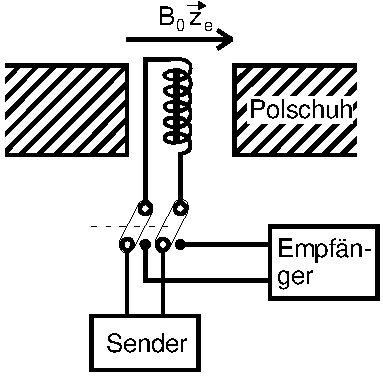
\includegraphics[width = 0.4\textwidth]{Pics/aufbau.pdf}
  \caption{Grundlegender Versuchsaufbau zur Bestimmung von $T_2$\cite{anleitung}.}
  \label{fig:aufbau}
\end{figure}
Der Abbau der Magnetisierung wird als freier Induktionszerfall (FID)
bezeichnet. Dieser kann prinzipiell durch Aufzeichnen der
Empfängersignale dargestellt werden.
Aufgrund von Nachbar-Spinwechselwirkungen und Inhomogenität in dem Magnetfeld des
Permanentmagneten treten Dephasierungsprozesse der Kernspins auf.
Aus diesem Grund fächert die Präzessionsbewegung der Spins
auf. Für die messbare Relaxationszeit $T^*_2$ gilt
\begin{equation}
  \label{eqn:T^*}
  \frac{1}{T^*_2} = \frac{1}{T_2} + \frac{1}{T_{\Delta B}}.
\end{equation}
Dabei ist $T_{\Delta B}$ eine apparative Zeitkonstante in der
Größenordnung von $\frac{1}{\gamma d G}$, wobei $d$ der Probendurchmesser
und $G$ der Gradient der Permanentmagnetfeldes.
Der freie Induktionszerfall zeigt bei dem Auftreten von mehreren
Resonanzstellen eine äußerst komplexe Struktur, die von der erwarteten
exponentiellen Form abweicht.
Ist das Permanentmagnetenfeld hinreichend homogen, ist
$T_{\Delta B}$ vernachlässigbar. In Fällen wo $T_{\Delta B} < T_2$
ist, ist die Bestimmung von $T_2$ durch die FID Methode nicht mehr möglich.

\subsubsection{Spin-Echo-Verfahren}
Die apparativ bedingten Effekte auf $T_2$ können eliminiert werden,
wenn diese Effekte zeitlich konstant sind. Das Spin-Echo-Verfahren
arbeitet mit zwei Pulsen. Der erste Puls ist ein 90°-Puls, mit
dem die Spins aus der $\vec{e}_z$-Achse gedreht werden.
Nun werden zwei Spins betrachtet, die aufgrund von Feldinhomogenitäten verschiedene Lamorfrequenzen
$\omega\ua{L, i}$ besitzen. Dabei sei o.B.d.A. $\omega\ua{L, 1} > \omega$ und
$\omega\ua{L, 2} < \omega$. Der Spin zu $\omega\ua{L, 1}$
dreht somit im Uhrzeigersinn in der $\vec{e}'_x$-$\vec{e}'_y$-Ebene.
Der zweite Spin läuft in der selben Ebene gegensinnig.
Das Spin-Echo-Verfahren ist zur Veranschaulichung in Abb.~\ref{eqn:spin_flip}
dargestellt.
Nach der Zeit $\tau$ kommt der zweite Puls. Dieser ist ein
180°-Puls mit dem der Spin um die $\vec{e}'_x$ gedreht wird.
Aus diesem Grund laufen die dephasierten Spins aufeinander zu, sodass
sie zum Zeitpunkt $2\tau$ in die selbe Richtung zeigen.
\begin{figure}[h]
  \centering
  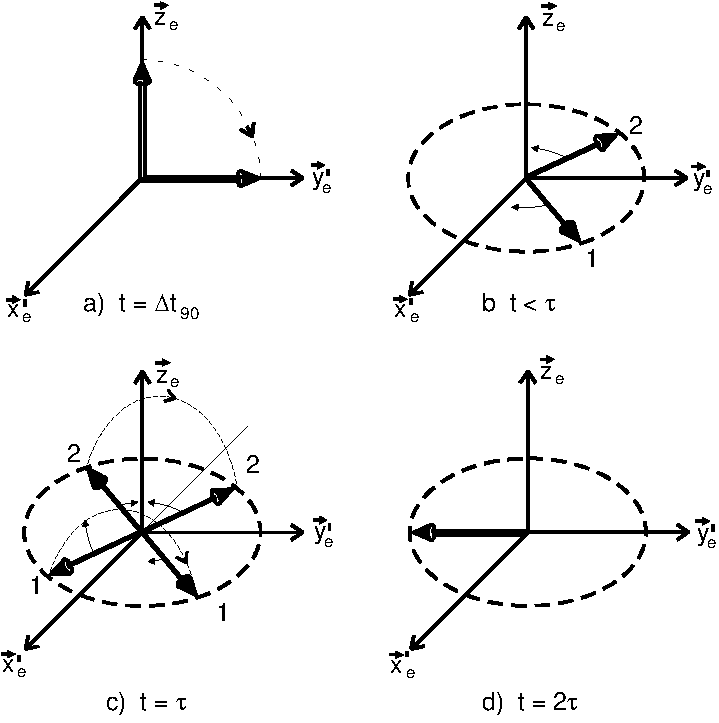
\includegraphics[width = 0.5\textwidth]{Pics/spin.pdf}
  \caption{Zeitliche Phasen des Spin-Echo-Verfahren\cite{anleitung}.}
  \label{eqn:spin_flip}
\end{figure}
Das Verfahren produziert das folgende Signal.
\begin{figure}[h]
  \centering
  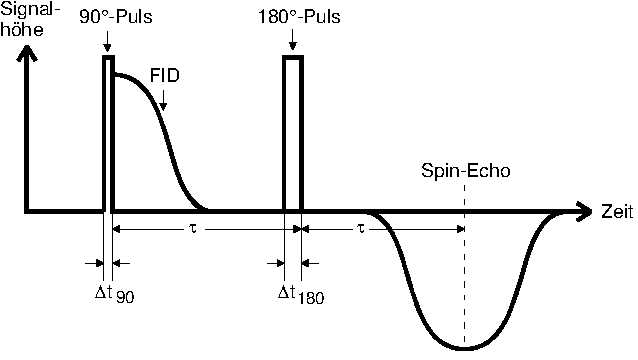
\includegraphics[width = 0.7\textwidth]{Pics/signalverlauf.pdf}
  \caption{Signalverlauf des Spin-Echo-Verfahrens\cite{anleitung}.}
  \label{eqn:signal}
\end{figure}
Neben den reversiblen Desphasierungsprozessen, welche mit dem Spin-Echo-Verfahren
vereinbar sind, gibt es irreversible Dephasierungsprozesse, die auf Wechselwirkungen
der Spins mit ihrer Umgebung basieren.
Daher nehmen nicht alle Spins am Echosignal teil, sodass bei zu groß gewählter Zeit $\tau$
die Amplitude des Echos signifikant kleiner wird.
Die Höhe der Spinechos klingt exponentiell ab.
Eine Veranschaulichung dieses Phänomens ist in Abb.~\ref{fig:dephase}
zu finden.
\begin{figure}[h]
  \centering
  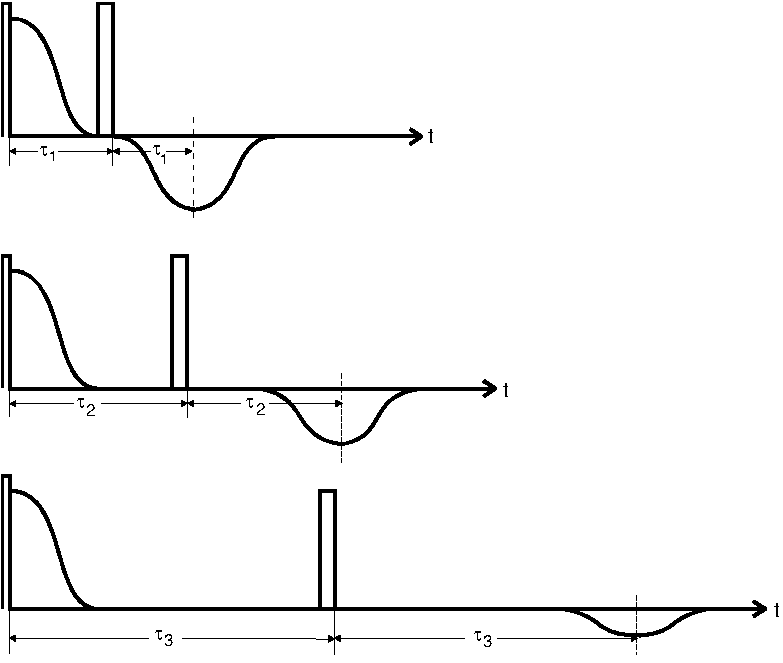
\includegraphics[width = 0.6\textwidth]{Pics/echo.pdf}
  \caption{Verkleinerung der Signalamplitude aufgrund von irreversiblen Dephasierungsprozessen
  für große $\tau$\cite{anleitung}.}
  \label{fig:dephase}
\end{figure}

\subsubsection{Carr-Purcell-Methode}
\vspace{-10pt}
Die Carr-Purcell-Methode ermöglicht durch Refokussierung das Vermessen von mehreren Spinechos
hintereinander. Dafür werden nach den beiden Pulsen des FID weitere 180°-Pulse
im Abstand von $2\tau$ eingespeist. Ist die Länge der einzelnen Pulse jedoch nicht
exakt eingestellt, werden die Pulse nicht mehr in die $x$-$y$-Ebene gedreht, sondern
liegen um einen Winkel $\delta$ außerhalb dieser.
Durch mehrfaches hintereinander Ausführen der fehlerhaften Pulslängen wird
der Fehler verstärkt.
\begin{figure}
  \centering
  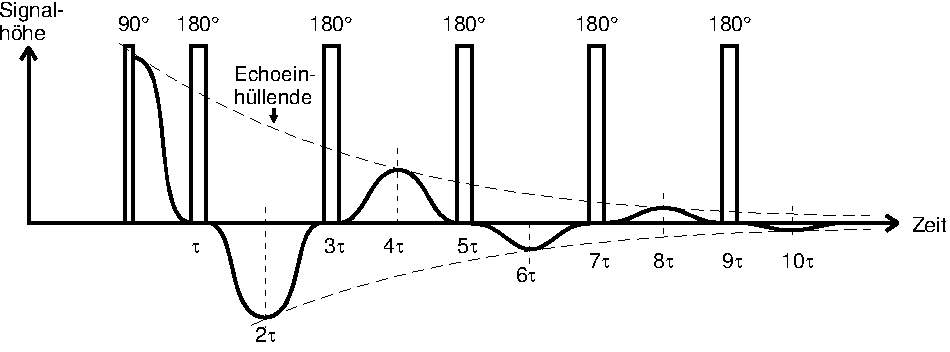
\includegraphics[width = 0.75\textwidth]{Pics/carr_purcell.pdf}
  \caption{Signalverlauf der Carr-Purcell-Methode\cite{anleitung}.}
  \label{eqn:carr_purcell}
\end{figure}
\vspace{-10pt}
\subsubsection{Meiboom-Gill-Methode}
\vspace{-15pt}
Die Verstärkung der Fehler wird in der Meiboom-Gill-Methode durch eine spezielle
Vorrichtung verhindert. Die Phase des 180°-Pulses wird um 90° gegenüber des
90°-Pulses Phasenverschoben. Alle $4\tau$ sind die Spins refokussiert in der
$y$-Richtung. Die Bewegung der Spins bei der beschriebenen Methode ist in
Abb.~\ref{fig:meiboom_gill} dargestellt.
\begin{figure}[h!]
  \centering
  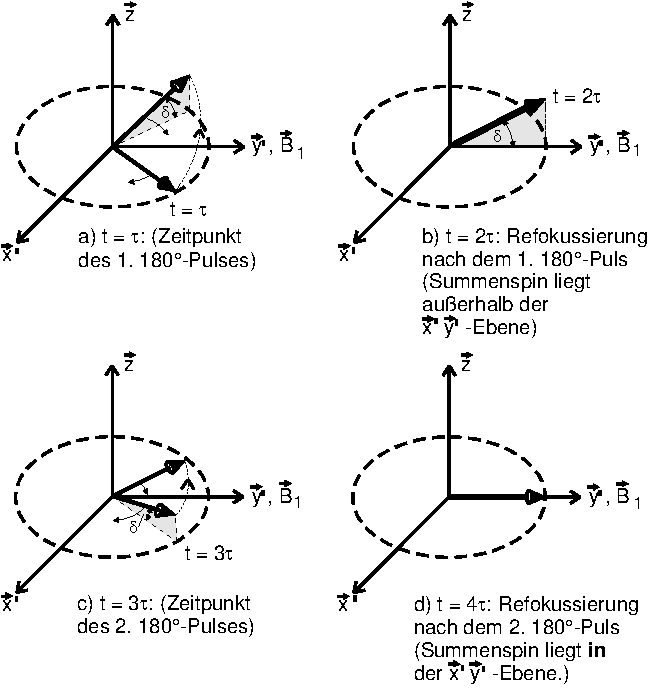
\includegraphics[width = 0.45\textwidth]{Pics/meiboom.pdf}
  \caption{Bewegung der Spins bei der Meiboom-Gill-Methode\cite{anleitung}.}
  \label{fig:meiboom_gill}
\end{figure}
\FloatBarrier
\subsection{Messmethode für $T_1$}
Die longitudinale Relaxationszeit $T_1$ wird ebenfalls mittels einer Pulsmethode
gemessen. Ein 180°-Puls dreht die Probenmagnetisierung aus ihrer Gleichgewichtslage
in die $-\vec{e}_z$-Richtung. Nach einer Zeit $\tau$ dreht ein 90°-Puls
den $\vec{e}_z$ Anteil der teilweise relaxierte Probenmagnetisierung
in die $x$-$y$-Ebene. Die Magnetisierung induziert in einer Spule eine Storm,
welcher proportional zu $\vec{M}(\tau)\cdot\vec{e}_y$ ist.
Die Blochschen Gleichungen~\eqref{eqn:M_x_relax}~bis~\eqref{eqn:M_z_relax}
ergeben für die Anfangsbedingungen $\vec{M}\cdot\vec{e}_x = \vec{M}\cdot\vec{e}_y = 0$
und $\vec{M}\cdot\vec{e}_z = -M_0$
\begin{equation}
  \label{eqn:zeit_mag}
  \vec{M}(\tau)\cdot\vec{e}_z = M_0\left(1-2\exp{\left(-\frac{\tau}{T_1}\right)}\right).
\end{equation}
Die Relaxationszeit $T_1$ kann durch Variation der Zeitkonstante $\tau$
aus einem Diagramm $\log{\left(\frac{M_0 - \vec{M}(\tau)\cdot\vec{e}_z}{2M_0}\right)}$
entnommen werden.

\subsection{Diffusion in einer flüssigen Probe}
Aufgrund der Brownschen Molekularbewegung diffundieren die
Kernspins in der flüssigen Probe umher, sodass sie aufgrund des inhomogenen
Magnetfeldes unterschiedliche Feldstärken unterliegen.
Dies hat zur Folge, dass die Lamor-Frequenz eine Funktion von der Zeit wird.
Explizite Rechnungen (vgl. \cite{anleitung}) führen darauf, dass die Magnetisierungsamplitude
der Spin-Echos exponentiell mit der Zeitkonstante
\begin{equation}
  \label{eqn:diffusion}
  T_{D} = \frac{3}{D\gamma^2G^2\tau^2}
\end{equation}
abnimmt.
In Formel~\eqref{eqn:diffusion} ist $D$ die Diffusionskonstante und $G$
der Magnetfeldgradient.
Für die zeitabhängige Magnetisierung ergibt sich
\begin{equation}
  \label{eqn:mag_diffusion}
  \vec{M}\cdot\vec{e}_y = M_0\exp{\left(\frac{-t}{T_2}\right)}\exp{\left(\frac{-t^3}{4T_{D}}\right)}.
\end{equation}

\subsection{Molekülradius}
Der Radius der Probenmoleküle kann mittels der Stokschen Formel
\begin{equation}
  \label{eqn:diffkonst}
  D = \frac{1}{6\beta\pi\eta r}
\end{equation}
berechnet werden. Die Viskosität $\eta$ der Probe wird mit Hilfe eines Kappilar-Viskosimeters
bei Normaldruck und Raumtemperatur bestimmt.

\section{Durchführung}
\subsection{Justage der Apparatur}
Zur Justage der Apparatur wird die Wasserprobe mit paramagnetischen Zentren (Kupfersulfat)
versetzt, sodass die Relaxationszeit verkürzt wird. Im Anschluss werden die Parameter
für den freien Induktionszerfall eingestellt.
Die Parameter werden iterativ gefunden. Die gefundenen geeigneten Parameter für die
Justageprobe ergeben sich zu
\begin{enumerate}
  \item A: $\SI{5,6}{\micro\second}$
  \item B: $\SI{10,12}{\micro\second}$
  \item $\omega$: $\SI{21,70806}{\mega\hertz}$
  \item $x$: -1,93
  \item $y$: -5,45
  \item $z$: 3,94
  \item $z^2$: -2,65
  \item Phase: 155°.
\end{enumerate}
Für die Probe des bidestillierten Wassers wurden die Parameter wie folgt angepasst.
\begin{enumerate}
  \item A: $\SI{5,2}{\micro\second}$
  \item B: $\SI{10,2}{\micro\second}$
  \item $\omega$: $\SI{21,70788}{\mega\hertz}$
\end{enumerate}

\subsection{Bestimmung von $T_1$}

Zunächst werden die Pulslängen A und B so eingestellt, dass zuerst der 180°-Puls und im
Anschluss erst der 90°-Puls auftritt. Es werden mehrere Werte im logarithmischen Abstand
genommen und die Spannungsmaxima des Signals auf einem Oszilloskop abgelesen und
auf einem USB-Stick gespeichert.

\subsection{Meiboom-Gill-Methode}

An der Apparatur wird der Schalter auf MG umgelegt. Die Anzahl der 180°-Pulse
wird ausreichend groß eingestllt, sodass der abklingende Signalverlauf der Spin-Echos
deutlich sichtibar ist. Die Abstände $\tau$ werden hinreichend klein gewählt, damit
der Einfluss der Diffusion minimiert wird.
Das Signal der Meiboom-Gill-Methode wird auf einem Oszilloskop abgebildet und mittels
eines USB-Sticks gespeichert.
Einen Signalverlauf der Carr-Purcell-Methode kann durch Abschalten des Schalters MG
sichtbar gemacht werden. Die Signalfolge wird ebenfalls auf einem USB-Stick gespeichert.

\subsection{Bestimmung der Diffusionskonstante}
Die Amplituden der Spin-Echos werden für verschiedene Zeiten $\tau$ bestimmt, wobei
darauf zu achten ist, die Wiederholungszeit auf ein Vielfaches von $T_1$ einzustellen.
Desweiteren wird die Halbwertsbreite $t_{\frac{1}{2}}$ der Spin-Echos bestimmt, damit der
Feldgradient ermittelt werden kann.
